\documentclass[10pt]{article}

%%%%%%%%%%%%%%%%%%%%%%%%%%%%%%%%%%%%%%%%%%%%%%%%%%%%%%%%%%%%%%%%%%%%%%%%%%%%%%%
%%% packages %%%
%%%%%%%%%%%%%%%%%%%%%%%%%%%%%%%%%%%%%%%%%%%%%%%%%%%%%%%%%%%%%%%%%%%%%%%%%%%%%%%

\usepackage[english]{babel} % Choose english language
\usepackage[labelfont = bf, font = small]{caption} % Use caption package. Use bold font for caption.
\usepackage{siunitx} % Use siunitx for unit representation.
\newcommand{\RM}[1]{\MakeUppercase{\romannumeral #1{:}}}
\usepackage{graphicx}
\usepackage{tabularx}
\usepackage{float}
\usepackage{lmodern}
\usepackage{filecontents}
\usepackage{amsmath}
\usepackage{amssymb}
\usepackage[utf8]{inputenc}
\usepackage[bottom]{footmisc}
\usepackage{leftidx}
\usepackage{subcaption}
\usepackage[explicit]{titlesec}
\usepackage{booktabs}
\usepackage{multirow}
\usepackage{multicol}
\usepackage{listings}
\usepackage{enumitem}
\usepackage{pgfplots}
\usepackage{natbib}
\usepackage{xcolor}
\usepackage{url}
\usepackage{array}
\usepackage{setspace}
\usepackage{hyperref} % Referencing
\usepackage{verbatim}
\usepackage{changepage}
\usepackage[footnote, printonlyused]{acronym}
\usepackage{scrextend}
\usepackage{geometry} % Change geometry of page layout
\usepackage{rotating}
\usepackage{longtable}
\usepackage{lscape}
\usepackage{tocloft}
\usepackage{tkz-euclide}
\usepackage{listings}
\usepackage{feynmp-auto} % Create fenynman diagrams
\usepackage{tikz-feynman} % Create fenynman diagrams
\usepackage{lipsum} % For testing. insert random text

%%%%%%%%%%%%%%%%%%%%%%%%%%%%%%%%%%%%%%%%%%%%%%%%%%%%%%%%%%%%%%%%%%%%%%%%%%%%%%%
%%% new commands and environments %%%
%%%%%%%%%%%%%%%%%%%%%%%%%%%%%%%%%%%%%%%%%%%%%%%%%%%%%%%%%%%%%%%%%%%%%%%%%%%%%%%

% Create custom font
\newenvironment{myfont}{\fontfamily{put}\selectfont}{\par}

% Adapt spacing between lines
%\doublespacing

% Delete dots from toc
\renewcommand{\cftdot}{}

% Change section label to roman
\renewcommand{\thesection}{\Roman{section}}

% Customize section layout
\newcommand{\ssection}[1]{%
  \section[#1]{\centering\normalfont\scshape #1}}
\newcommand{\ssubsection}[1]{%
  \subsection[#1]{\centering\normalfont\itshape #1}}
\newcommand{\ssubsubsection}[1]{%
  \subsubsection[#1]{\centering\normalfont #1}}

% Import tikz libraries for figures
\usetikzlibrary{positioning,shadows,arrows}

% Create footnotereferencing
\makeatletter
\newcommand\footnoteref[1]{\protected@xdef\@thefnmark{\ref{#1}}\@footnotemark}
\makeatother

% Change layout of page
\hypersetup{
  colorlinks = true,
  linkbordercolor = {red},
  citebordercolor = {red},
  menubordercolor = {blue},
  urlbordercolor = {blue},
  linktoc = {page},
  pagebackref = {True},
  pdftitle = {Solution 11},
  pdfauthor = {Nils Hoyer, Maurice Morgenthaler},
  pdfcreator  = {pdflatex},
  pdfproducer = {LaTeX}
}

% Change geometry of page
\geometry{a4paper, top = 20mm, left = 20mm, right = 20mm, bottom = 15mm, headsep = 8mm, footskip = 10mm, includeheadfoot}

% Decalre uits for SIunitx
\DeclareSIUnit\femtobarn{fb^{-1}}
\DeclareSIUnit\percent{\%}

% Define colors
\definecolor{deepblue}{rgb}{0,0,0.5}
\definecolor{deepred}{rgb}{0.6,0,0}
\definecolor{deepgreen}{rgb}{0,0.6,0.2}
\definecolor{deeporange}{rgb}{0.9,0.2,0}

% Commands for further use
\newcommand{\testStat}{\tilde{q}_{\mu}}
\newcommand{\lL}[2]{\mathcal{L}\left(#1 \middle|#2 \right)}
\newcommand{\likelihood}{\mathfrak{L}}
%%%%%%%%%%%%%%%%%%%%%%%%%%%%%%%%%%%%%%%%%%%%%%%%%%%%%%%%%%%%%%%%%%%%%%%%%%%%%%%
%%% start document %%%
%%%%%%%%%%%%%%%%%%%%%%%%%%%%%%%%%%%%%%%%%%%%%%%%%%%%%%%%%%%%%%%%%%%%%%%%%%%%%%%

\begin{document}
\begin{myfont}
\lstset{language=C++,
  basicstyle=\ttfamily,
  keywordstyle=\color{blue}\ttfamily,
  stringstyle=\color{red}\ttfamily,
  commentstyle=\color{green}\ttfamily,
  morecomment=[l][\color{magenta}]{\#}
}

\begin{center}
  \begin{Large}
    \textsc{Solution for homework assignment no. 11} \\
  \end{Large}
  \vspace*{0.4cm}
    Nils Hoyer, Maurice Morgenthaler
  \vspace*{1cm}
\end{center}

\section*{Exercise 11.1}

\begin{itemize}
	\item[\textbf{a)}] Given a Poissonian distribution with mean $\nu$
	
	\begin{equation}
		f_{n}(\nu) = e^{-n}\frac{n^{\nu}}{\nu\,!}
	\end{equation}

	\noindent we are asked to list the number of observed events such that there is a \SI{10}{\percent} chance to observe them above, below and outside of the central interval. \\
	As usual, please find the code in file \texttt{exercise11\_1a.C}.
	The results are given in table \ref{tab:ex1_results_a}.

	\begin{longtable}{*{14}l}
		\endfirsthead
		\endhead
		\toprule
		\textbf{Exercise} & \textbf{$\nu$} & 1 & 2 & 3 & 4 & 5 & 6 & 7 & 8 & 9 & 10 & 11 & 12 \\
		\midrule
		\textbf{1}                  & \multirow{2}{*}{\textbf{n}} & 5 & 5 & 6 & 8 & 9  & 10 & 11 & 13 & 14 & 15 & 16 & 18 \\ \cline{3-14}
		\textbf{2}                  &                             & 1 & 1 & 2 & 3 & 3  & 4  & 5  & 6  & 6  & 7  & 8  & 9  \\ \cline{2-14}
		\multirow{2}{*}{\textbf{3}} & \textbf{n'}                 & 1 & 1 & 2 & 2 & 3  & 3  & 4  & 5  & 5  & 6  & 7  & 8  \\ \cline{3-14}
		                            & \textbf{n}                  & 4 & 6 & 7 & 9 & 10 & 11 & 13 & 14 & 15 & 16 & 18 & 19 \\
		\bottomrule
		\caption[]{Results obtained for a fixed mean $\nu$.}
		\label{tab:ex1_results_a}
	\end{longtable}

	\item[\textbf{b)}] Similar to the first part we are asked to calculatze the \SI{90}{\percent} CL for $\nu$ given the total number of observed events $n$. \\
	As usual, please find the code in file \texttt{exercise11\_1b.C}.
	The results are given in table \ref{tab:ex1_results_b}.
	
	\begin{longtable}{*{15}l}
		\endfirsthead
		\endhead
		\toprule
		\textbf{Exercise} & \textbf{$n$} & 0 & 1 & 2 & 3 & 4 & 5 & 6 & 7 & 8 & 9 & 10 & 11 & 12 \\
		\midrule
		\textbf{1}                  & \multirow{2}{*}{\textbf{$\nu$}} & 2.30 & 3.89 & 5.32 & 6.68 & 7.99 & 9.28 & 10.5 & 11.77 & 13.00 & 14.21 & 15.41 & 16.60 & 17.78 \\ \cline{3-15}
		\textbf{2}                  &                             & 0.11 & 0.53 & 1.10 & 1.75 & 2.43 & 3.15 & 3.90 & 4.66 & 5.43 & 6.22 & 7.02 & 7.83 & 8.65 \\ \cline{2-15}
		\multirow{2}{*}{\textbf{3}} & \textbf{$\nu$'}                 & 0.05 & 0.36 & 0.82 & 1.37 & 1.97 & 2.61 & 3.29 & 3.98 & 4.70 & 5.43 & 6.17 & 6.93 & 7.69 \\ \cline{3-15}
		                            & \textbf{$\nu$}                  & 3.00 & 4.74 & 6.30 & 7.75 & 9.15 & 10.51 & 11.84 & 13.15 & 14.44 & 15.71 & 16.96 & 18.21 & 19.44 \\
		\bottomrule
		\caption[]{Results obtained for a fixed number of events $n$.}
		\label{tab:ex1_results_b}
	\end{longtable}
\end{itemize}

\section*{Exercise 11.2}
\label{sec:11_2}

Given the total number of observed events $n_{\textrm{tot}} = n_{\textrm{S}} + n_{\textrm{B}}$ where $n_{\textrm{S}}$ is the number of signal and $n_{\textrm{B}}$ the number of background events we are asked to derive an upper limit for the mean $\nu_{\textrm{S}}$ at the \SI{95}{\percent} confidence limit.
We also know that $\nu_{\textrm{B}}$ and that $n$ follows a Poissonian distribution. \\
To answer this question we relate the upper limit with respect to a Poissonian distribution and the quantile of the $\chi^{2}$ distribution such that

\begin{equation}
	s_{\textrm{up}} = \frac{1}{2} \textrm{F}_{\chi^{2}}^{-1}\left[p, 2(n+1)\right] - b.
\end{equation}

\noindent This is possible because of the relation between the cumulative Poissonian distribution and the cumulative $\chi^{2}$ distribution.

\begin{equation}
	\textrm{Pr}(X = k) = \textrm{F}_{\chi^{2}}(2\lambda; 2(k+1)) - \textrm{F}_{\chi^{2}}(2\lambda; 2k)
\end{equation}

\noindent The implementation into code is given in file \texttt{exercise11\_2.C}. \\
Using $n_{obs} =$ \num{5} yields $\nu_{S}^{max} \approx$ \num{8.73096}.


\section*{Exercise 11.3}

We are asked to verify the value obtained in exercise \ref{sec:11_2}.
To do this we use \num{10000} toy Monte Carlo experiments to generate random variables according to a Poissonian distribution with mean $\nu = \nu_{\textrm{B}} + \nu_{\textrm{S}}^{\textrm{max}}$ where $\nu_{\textrm{S}}^{\textrm{max}}$ is used from exercise 11.2.
By construction the number of events $< n_{\textrm{obs}}$ should be \SI{5}{\percent}. \\
The implementation into code is given in file \texttt{exercise11\_3.C}.
The plot showing the results is given in figure \ref{fig:ex11_3_results}.

\begin{figure}
	\centering
	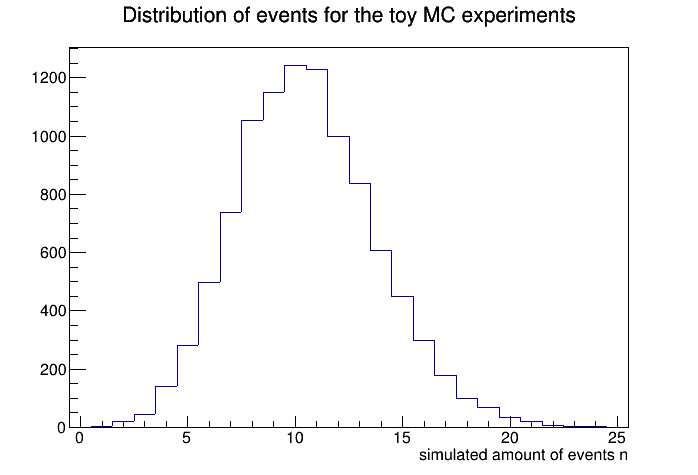
\includegraphics[width = 0.6 \textwidth]{./exercise11_3.png}
	\caption{Results from our \num{10000} Monte Carlo simulation of $n$.}
\end{figure}

\noindent Using the value given in exericse \ref{sec:11_2} we get a fraction of $n$ which is observed below $n_{obs} =$ \num{5} of \SI{4.89}{\percent} which does not disagree with the expected value of \SI{5}{\percent}.

\end{myfont}
\end{document}